\documentclass[10pt,a4paper]{article}

% Packages
\usepackage{fancyhdr}           % For header and footer
\usepackage{multicol}           % Allows multicols in tables
\usepackage{tabularx}           % Intelligent column widths
\usepackage{tabulary}           % Used in header and footer
\usepackage{hhline}             % Border under tables
\usepackage{graphicx}           % For images
\usepackage{xcolor}             % For hex colours
%\usepackage[utf8x]{inputenc}    % For unicode character support
\usepackage[T1]{fontenc}        % Without this we get weird character replacements
\usepackage{colortbl}           % For coloured tables
\usepackage{setspace}           % For line height
\usepackage{lastpage}           % Needed for total page number
\usepackage{seqsplit}           % Splits long words.
%\usepackage{opensans}          % Can't make this work so far. Shame. Would be lovely.
\usepackage[normalem]{ulem}     % For underlining links
% Most of the following are not required for the majority
% of cheat sheets but are needed for some symbol support.
\usepackage{amsmath}            % Symbols
\usepackage{MnSymbol}           % Symbols
\usepackage{wasysym}            % Symbols
%\usepackage[english,german,french,spanish,italian]{babel}              % Languages
\usepackage{fontawesome}

% Document Info
\author{FFY00}
\pdfinfo{
  /Title (Assembly for Reverse Engeneering Cheat Sheet)
  /Author (FFY00)
}

% Lengths and widths
\addtolength{\textwidth}{8cm}
\addtolength{\textheight}{-1cm}
\addtolength{\hoffset}{-4cm}
\addtolength{\voffset}{-2.5cm}
\setlength{\tabcolsep}{0.2cm} % Space between columns
%\setlength{\headsep}{-12pt} % Reduce space between header and content
%\setlength{\headheight}{85pt} % If less, LaTeX automatically increases it
\renewcommand{\footrulewidth}{0pt} % Remove footer line
\renewcommand{\headrulewidth}{0pt} % Remove header line
\renewcommand{\seqinsert}{\ifmmode\allowbreak\else\-\fi} % Hyphens in seqsplit
% This two commands together give roughly
% the right line height in the tables
\renewcommand{\arraystretch}{1.3}
\onehalfspacing
\pagenumbering{gobble} % Remove page number

% Commands
\newcommand{\SetRowColor}[1]{\noalign{\gdef\RowColorName{#1}}\rowcolor{\RowColorName}} % Shortcut for row colour
\newcommand{\mymulticolumn}[3]{\multicolumn{#1}{>{\columncolor{\RowColorName}}#2}{#3}} % For coloured multi-cols
\newcolumntype{x}[1]{>{\raggedright}p{#1}} % New column types for ragged-right paragraph columns
\newcommand{\tn}{\tabularnewline} % Required as custom column type in use

% Font and Colours
\definecolor{HeadBackground}{HTML}{333333}
\definecolor{FootBackground}{HTML}{666666}
\definecolor{TextColor}{HTML}{333333}
\definecolor{DarkBackground}{HTML}{248F24}
\definecolor{LightBackground}{HTML}{D9EBD9}
\renewcommand{\familydefault}{\sfdefault}
\color{TextColor}

\begin{document}
\raggedright
\raggedcolumns
\thispagestyle{empty}
\vspace*{-80pt}
\hspace*{-80pt}
\enlargethispage{200pt}

% Set font size to small. Switch to any value
% from this page to resize cheat sheet text:
% www.emerson.emory.edu/services/latex/latex_169.html
\small % Small font.

\begin{multicols}{3}

\begin{tabularx}{6cm}{p{1 cm} x{4.6 cm} }
\SetRowColor{DarkBackground}
\mymulticolumn{2}{x{6cm}}{\bf\textcolor{white}{\faGears\space General Registers}}  \tn
% Row 0
\SetRowColor{LightBackground}
EAX & Accumulator \tn 
% Row Count 1 (+ 1)
% Row 1
\SetRowColor{white}
EBX & Base \tn 
% Row Count 2 (+ 1)
% Row 2
\SetRowColor{LightBackground}
ECX & Counter \tn 
% Row Count 3 (+ 1)
% Row 3
\SetRowColor{white}
EDX & Data \tn 
% Row Count 4 (+ 1)
\hhline{>{\arrayrulecolor{DarkBackground}}--}
\end{tabularx}
\par\addvspace{1.3em}

\begin{tabularx}{6cm}{p{0.5 cm} x{5.1 cm} }
\SetRowColor{DarkBackground}
\mymulticolumn{2}{x{6cm}}{\bf\textcolor{white}{\faGears\space Pointer Registers}}  \tn
% Row 0
\SetRowColor{LightBackground}
ESP & Stack Pointer, "top" of the current stack frame (lower memory) \tn 
% Row Count 2 (+ 2)
% Row 1
\SetRowColor{white}
EBP & Base Pointer, "bottom" of the current stack frame (higher memory) \tn 
% Row Count 4 (+ 2)
% Row 2
\SetRowColor{LightBackground}
EIP & Instruction Pointer, pointer to the  next  instruction to  be executed by the CPU \tn 
% Row Count 7 (+ 3)
\hhline{>{\arrayrulecolor{DarkBackground}}--}
\end{tabularx}
\par\addvspace{1.3em}

\begin{tabularx}{6cm}{p{0.5 cm} x{5.1 cm} }
\SetRowColor{DarkBackground}
\mymulticolumn{2}{x{6cm}}{\bf\textcolor{white}{\faGear\space Index Registers}}  \tn
% Row 0
\SetRowColor{LightBackground}
ESI & Source Index, it is used as source index for string operations \tn 
% Row Count 2 (+ 2)
% Row 1
\SetRowColor{white}
EDI & Destination Index, it is used as destination index for string operations \tn 
% Row Count 4 (+ 2)
\hhline{>{\arrayrulecolor{DarkBackground}}--}
\end{tabularx}
\par\addvspace{1.3em}

\begin{tabularx}{6cm}{p{0.5 cm} x{5.1 cm} }
\SetRowColor{DarkBackground}
\mymulticolumn{2}{x{6cm}}{\bf\textcolor{white}{\faFlag\space Flags Registers}}  \tn
% Row 0
\SetRowColor{LightBackground}
ZF & Zero Flag, set when result of an operation equals zero \tn 
% Row Count 2 (+ 2)
% Row 1
\SetRowColor{white}
CF & Carry Flag, set when the result of an operation is too large/small \tn 
% Row Count 4 (+ 2)
% Row 2
\SetRowColor{LightBackground}
SF & Sign Flag, set when the result of an operation is negative \tn 
% Row Count 6 (+ 2)
\hhline{>{\arrayrulecolor{DarkBackground}}--}
\end{tabularx}
\par\addvspace{1.3em}

\begin{tabularx}{6cm}{X}
\SetRowColor{DarkBackground}
\mymulticolumn{1}{x{6cm}}{\bf\textcolor{white}{\faSortAmountDesc\space Stack}}  \tn
\SetRowColor{LightBackground}
\mymulticolumn{1}{p{6cm}}{\vspace{1px}\centerline{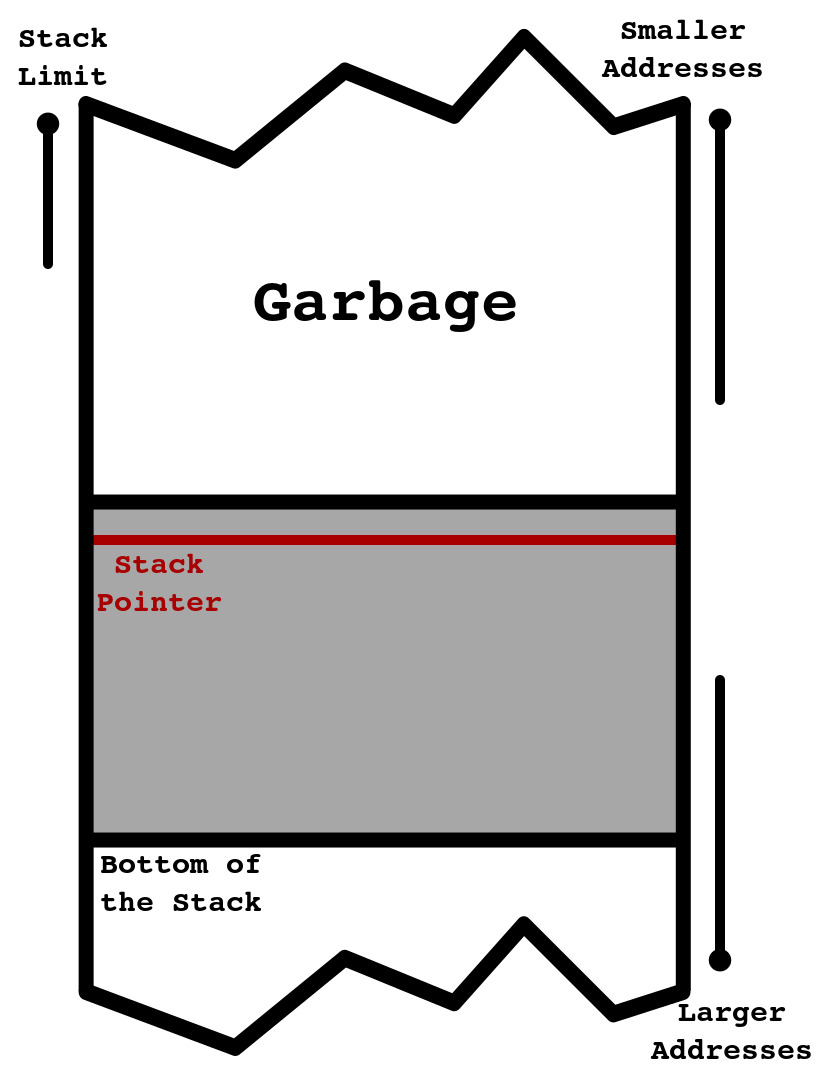
\includegraphics[width=5.5cm]{stack.png}}} \tn 
\hhline{>{\arrayrulecolor{DarkBackground}}-}
\SetRowColor{LightBackground}
\mymulticolumn{1}{x{6cm}}{Stack is a LIFO-Storage (Last In First Out)}  \tn 
\hhline{>{\arrayrulecolor{DarkBackground}}-}
\end{tabularx}
\par\addvspace{1.3em}

\begin{tabularx}{6cm}{x{2 cm} x{3.6 cm} }
\SetRowColor{DarkBackground}
\mymulticolumn{2}{x{6cm}}{\bf\textcolor{white}{\faExchange\space Moving Data}}  \tn
% Row 0
\SetRowColor{LightBackground}
mov ebx, eax & Move the value in {\emph{EAX}} to {\emph{EBX}} \tn 
% Row Count 2 (+ 2)
% Row 1
\SetRowColor{white}
mov eax, 0xDEADBEEF & Move {\emph{0xDEADBEEF}} into {\emph{EAX}} \tn 
% Row Count 4 (+ 2)
% Row 2
\SetRowColor{LightBackground}
mov edx, DWORD PTR {[}0x41424344{]} & Move the 4-byte value at address {\emph{0x41424344}} into {\emph{EDX}} \tn 
% Row Count 7 (+ 3)
% Row 3
\SetRowColor{white}
mov ecx, DWORD PTR {[}edx{]} & Move the 4-byte value at the address in {\emph{EDX}}, into {\emph{ECX}} \tn 
% Row Count 10 (+ 3)
% Row 4
\SetRowColor{LightBackground}
mov eax, DWORD PTR {[}ecx+esi*8{]} & Move the value at the address {\emph{ECX+ESI*8}} into {\emph{EAX}} \tn 
% Row Count 13 (+ 3)
% Row 5
\SetRowColor{white}
mov bx, 0C3EEh & Sign bit of {\emph{BL}} is now {\emph{1}}: {\emph{BH == 1100 0011}}, {\emph{BL == 1110 1110}} \tn 
% Row Count 16 (+ 3)
% Row 6
\SetRowColor{LightBackground}
movsx ebx, bx & Load signed 16-bit value into 32-bit register and sign-extend \tn 
% Row Count 19 (+ 3)
% Row 7
\SetRowColor{white}
movzx dx, bl & Load unsigned 8-bit value into 16-bit register and zero-extend \tn 
% Row Count 22 (+ 3)
% Row 8
\SetRowColor{LightBackground}
lea edi, {[}esi+0Bh{]} & Add {\emph{11}} to {\emph{ESI}} and store the result in {\emph{EDI}} \tn 
% Row Count 25 (+ 3)
\hhline{>{\arrayrulecolor{DarkBackground}}--}
\SetRowColor{LightBackground}
\mymulticolumn{2}{x{6cm}}{{\emph{eax}} is the value stored in eax \newline {\emph{{[}eax{]}}} is the value pointed to by eax}  \tn 
\hhline{>{\arrayrulecolor{DarkBackground}}--}
\end{tabularx}
\par\addvspace{1.3em}

\begin{tabularx}{6cm}{x{3 cm} x{2.6 cm} }
\SetRowColor{DarkBackground}
\mymulticolumn{2}{x{6cm}}{\bf\textcolor{white}{\faList\space Data Types}}  \tn
% Row 0
\SetRowColor{LightBackground}
BYTE & 1 Byte (8 bits) \tn 
% Row Count 1 (+ 1)
% Row 1
\SetRowColor{white}
WORD & 2 Bytes (16 bits) \tn 
% Row Count 2 (+ 1)
% Row 2
\SetRowColor{LightBackground}
DOUBLE WORD & 4 Bytes (32 bits) \tn 
% Row Count 3 (+ 1)
% Row 3
\SetRowColor{white}
QUAD WORD & 8 Bytes (64 bits) \tn 
% Row Count 4 (+ 1)
\hhline{>{\arrayrulecolor{DarkBackground}}--}
\end{tabularx}
\par\addvspace{1.3em}

\begin{tabularx}{6cm}{x{0.7 cm} x{4.9 cm} }
\SetRowColor{DarkBackground}
\mymulticolumn{2}{x{6cm}}{\bf\textcolor{white}{\faWrench\space Frequent Instructions}}  \tn
% Row 0
\SetRowColor{LightBackground}
mov & MOV is the instruction used for assignment. MOV can move data between a register and memory. \tn 
% Row Count 4 (+ 4)
% Row 1
\SetRowColor{white}
movsx & {\emph{move with Sign Extension}}. The data is moved from a smaller register into a bigger register, and the sign is preserved. \tn 
% Row Count 9 (+ 5)
% Row 2
\SetRowColor{LightBackground}
movzx & {\emph{move with Zero Extension}}. The data is moved from a smaller register into a bigger register, and the sign is ignored. \tn 
% Row Count 14 (+ 5)
% Row 3
\SetRowColor{white}
lea & Similar to MOV, except that math can be done on the original value before it is used. The {\emph{{[}}} and {\emph{{]}}} characters always surround the second parameter, but in this case they do {\bf{not indicate dereferencing}}. \tn 
% Row Count 22 (+ 8)
% Row 4
\SetRowColor{LightBackground}
push & Decrements the stack pointer by the size of the operand, then saves the operand to the new address. Equivalent to `sub esp, 4 | mov DWORD PTR {[}esp{]}, ebx` \tn 
% Row Count 28 (+ 6)
% Row 5
\SetRowColor{white}
pop & Sets the operand to the value on the stack, then increments the stack pointer by the size of the operand. Equivalent to `mov ebx, DWORD PTR {[}esp{]} | add esp, 4` \tn 
% Row Count 34 (+ 6)
% Row 6
\SetRowColor{LightBackground}
cmp & Compares two operands and sets or unsets flags in the flags register based on the result. \tn 
% Row Count 4 (+ 4)
% Row 7
\SetRowColor{white}
test & Bitwise AND. \tn 
% Row Count 5 (+ 1)
% Row 8
\SetRowColor{LightBackground}
rep, repnz, repz & Repeat while Equal/Non Zero/Zero. \tn 
% Row Count 7 (+ 2)
\hhline{>{\arrayrulecolor{DarkBackground}}--}
\end{tabularx}
\par\addvspace{1.3em}

% That's all folks
\end{multicols}

\end{document}
